%%%%%%%%%%%%%%%%%%%%%%%%%%%%%%%%%%%%%%%%%%%%%%%%%%%%%%%%%%%%%%%%%%%%%%%%%%%%%%%%%%%%%%
% Digitaler Designe-Flow               
%%%%%%%%%%%%%%%%%%%%%%%%%%%%%%%%%%%%%%%%%%%%%%%%%%%%%%%%%%%%%%%%%%%%%%%%%%%%%%%%%%%%%%
\section{Digitaler Designe-Flow}

\begin{minipage}{0.35\textwidth}
	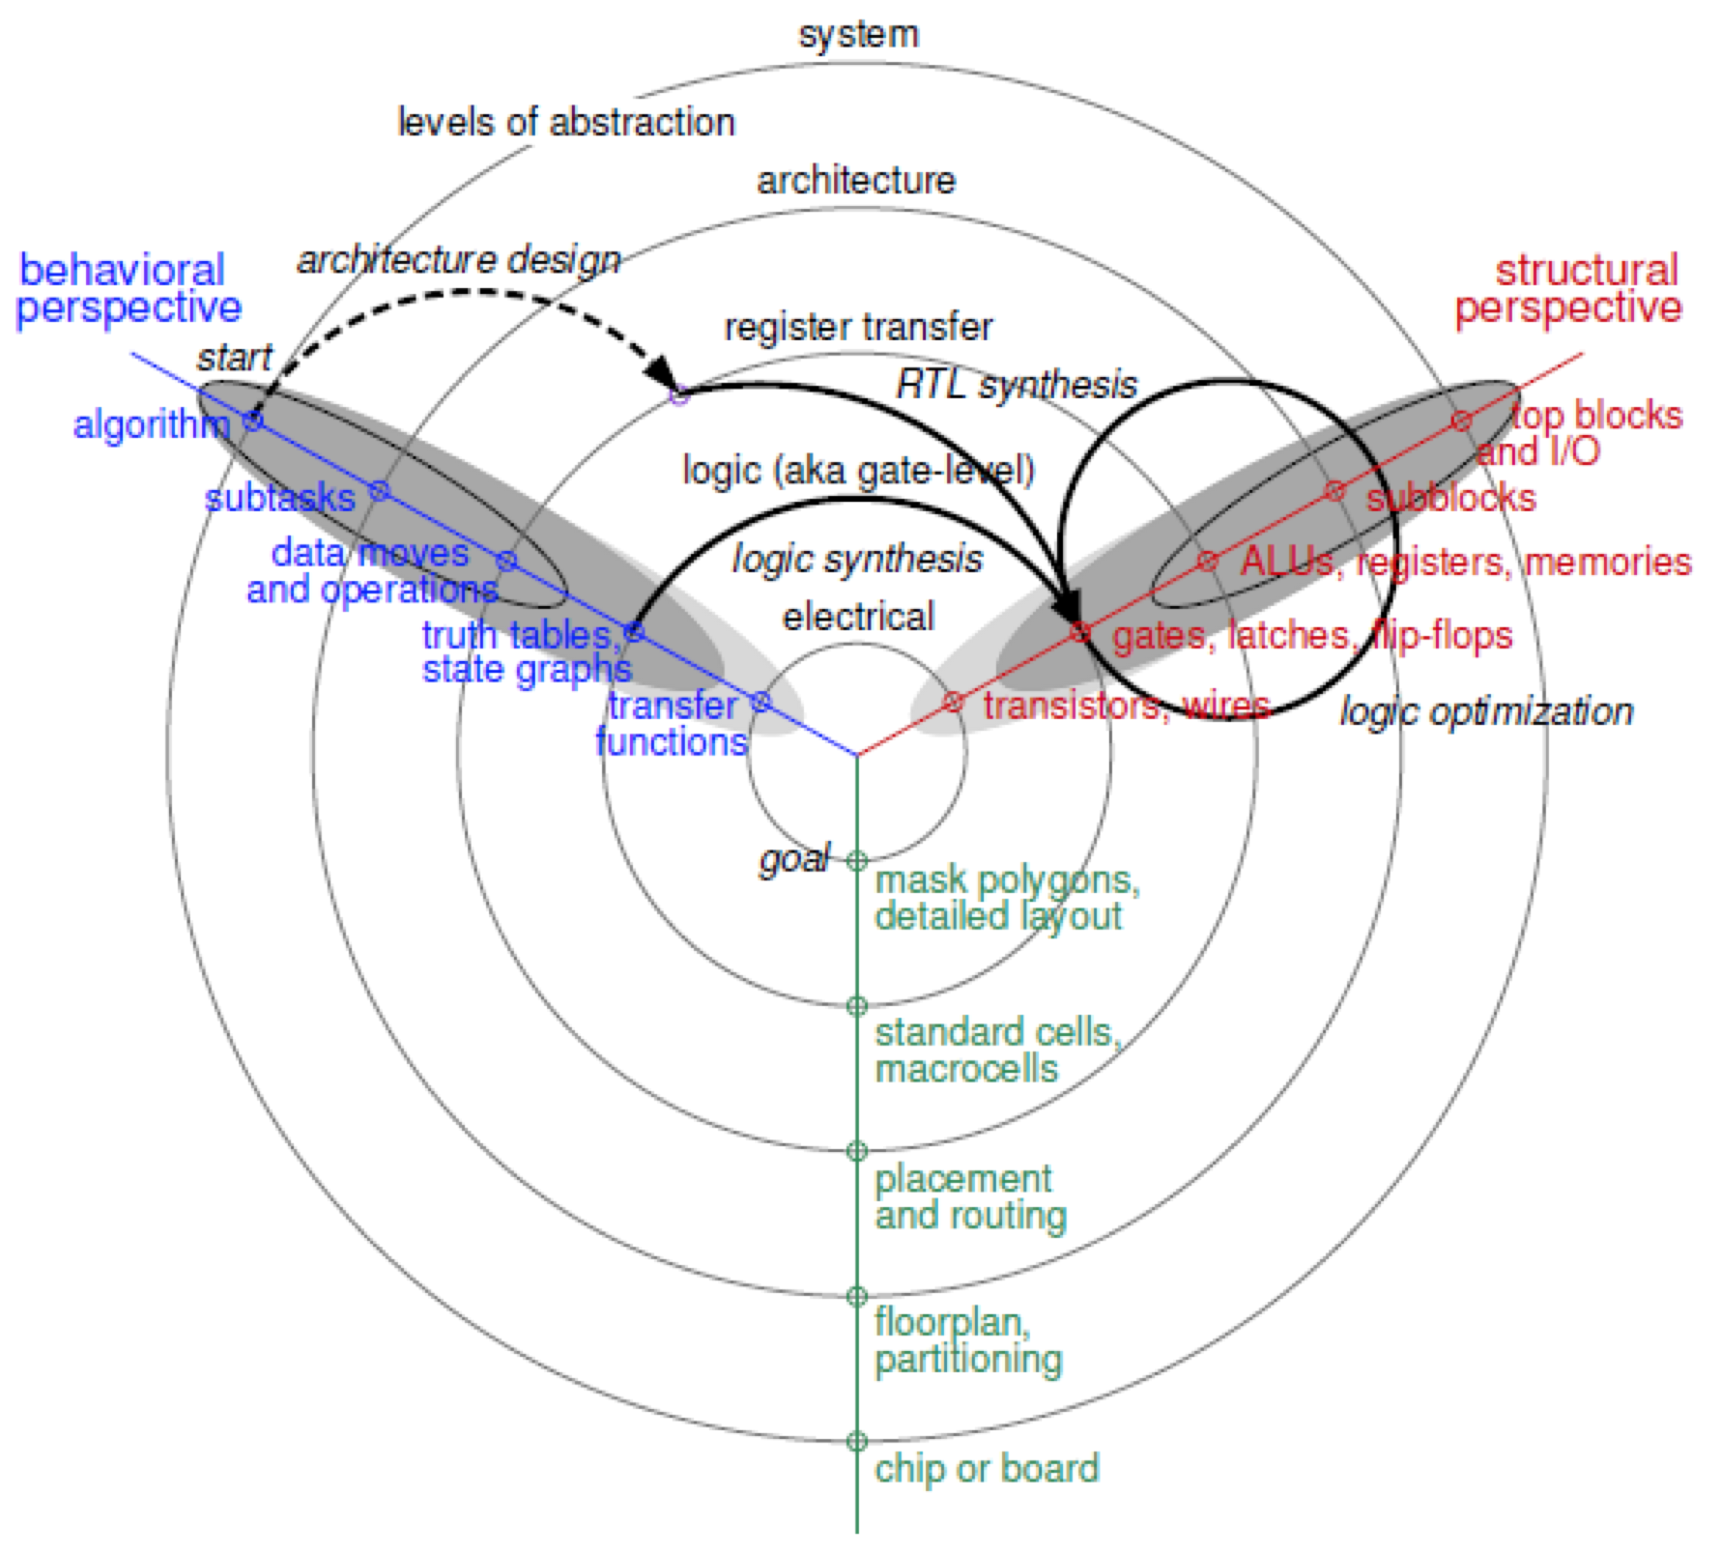
\includegraphics[width=\textwidth]{./bilder/Gajshi}
\end{minipage}
\begin{minipage}{0.6\textwidth}
	\begin{tabular}{l l }
		\multicolumn{2}{l}{\textbf{Y-Model von Gajski}}\\
		1. Verhaltenssicht (blau)		& $\rightarrow$ Wie muss sich das System Verhalten? \\
		2. Struckturelle Sicht (rot)	& $\rightarrow$ Welche elektronische Schaltungen/Baublöcke\\
		3. Physikalische Sicht (grün)	& $\rightarrow$ Wo und wie platziere ich meine Blöcke?\\
	\end{tabular}
	
	\subsection{Desigenprozess}
	\begin{enumerate}
		\item Wichtigste Fragen:
		\begin{itemize}
			\item Welches verhalten will der Kunde
			\item Gewünschte Schnittstellen 
			\item Randbedingungen: Grösse, Kosten, \dots
			\item Soft-, Hardware oder mixed Lösung gewünscht 
			\item Gibt es schon etwas ähnliches auf dem Markt
			\item \dots
		\end{itemize}
	\end{enumerate}
\end{minipage}

\begin{enumerate}
	\setcounter{enumi}{1}
	\item Sobald der Hardwareblock bekannt ist kann man mit dem digitalen Entwurfsprozess starten 
	\item Verhalten werden Verfeinert, Algorithmen zerlegt und in Strukturelle Ebenen übersetzt	
\end{enumerate}

\newpage

\begin{minipage}{.6\textwidth}
	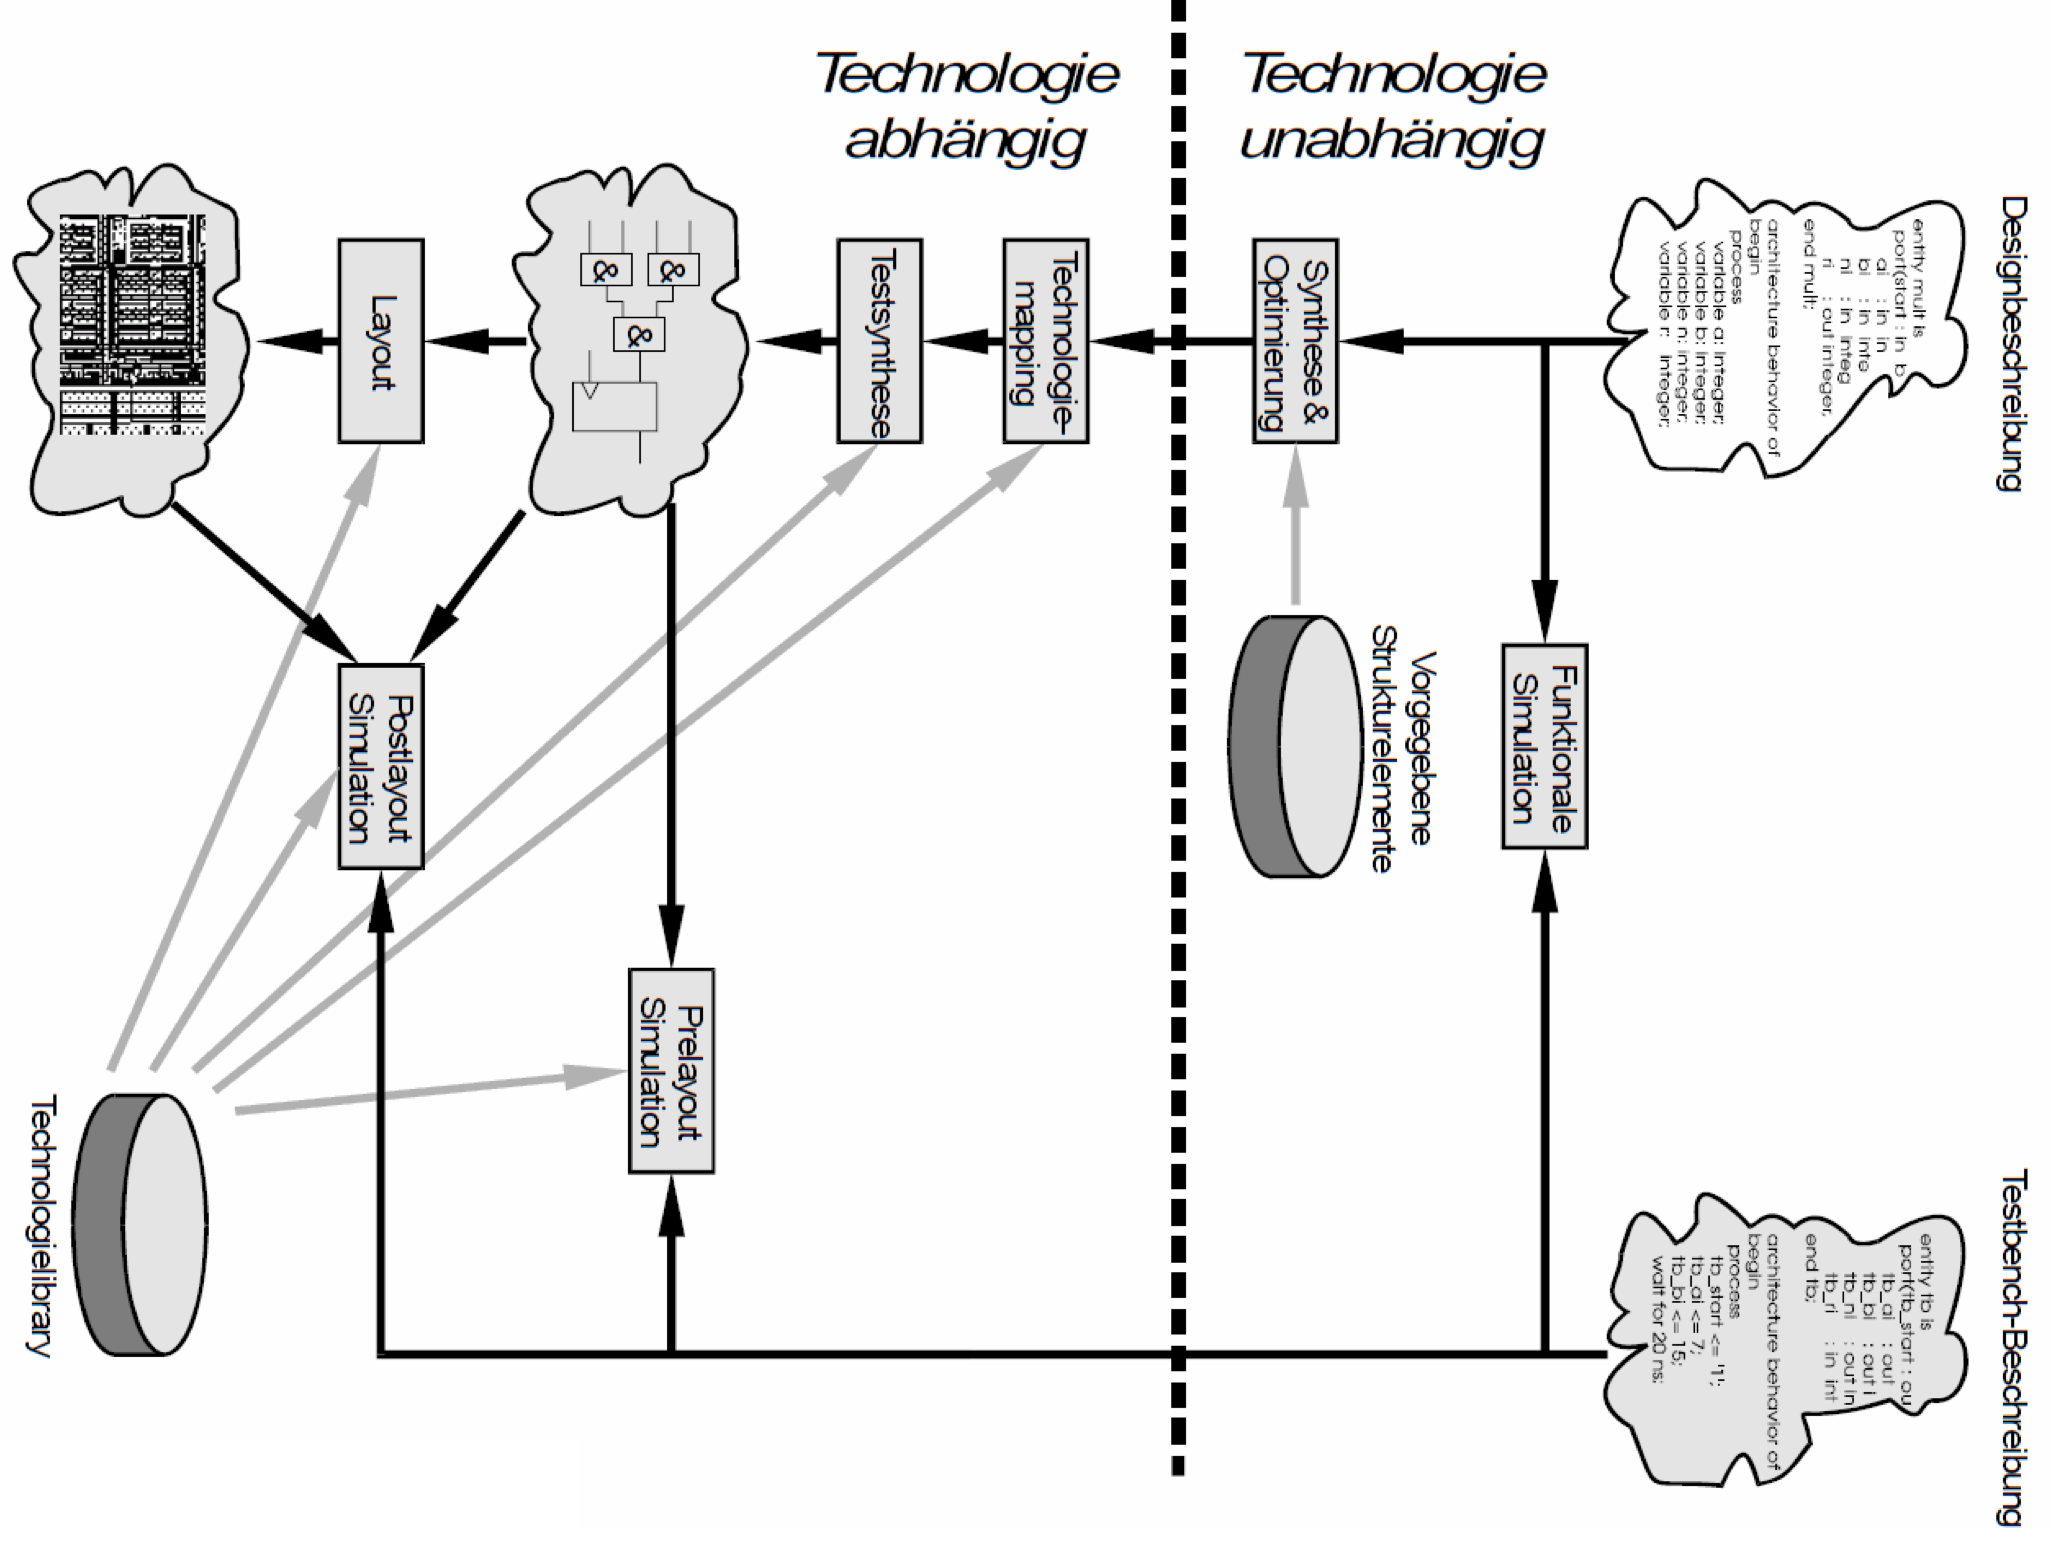
\includegraphics[width=\textwidth]{./bilder/FlowDesigen}
\end{minipage}
\begin{minipage}{.4\textwidth}
	\begin{tabular}{l}
		1. Designbeschreibung\\
		\quad $\rightarrow$ in VHDL \\
		2. Synthese und Optimierung\\
		\quad $\rightarrow$ Übersetzung in generische Netzliste {\tiny(noch kein timing)}\\
		3. Tegnologie Mapping\\
		\quad $\rightarrow$ auf real existierende Baublöcke anpassen\\
		4. Place \& Route\\
		\quad $\rightarrow$ Hardware wird "Programmiert"' (real timing)\\
		5. Simulation \\
		\quad $\rightarrow$ mit Hilfe einer Test-Bench {\tiny(meistens mit einem Zeitdiagramm)}\\
	\end{tabular}
\end{minipage}